%!TEX root=../../main.tex

\section{Backend - REST-Schnittstelle und Infrastruktur}
\label{chap:backendsota}
	\subsection{Einleitung}
	Das Backend besteht aus mehreren Komponenten. Einerseits soll eine gewisse System-Infrastruktur aufgebaut werden, um das \gls{webinterface} und die REST-Schnittstelle bereitzustellen. Andererseits muss die Anwendung selbst entwickelt werden. Diese besteht aus mehreren Teilen. Darunter fällt die REST-Schnittstelle, inklusive der implementierten Endpoints, Schnittstellen zu diversen Diensten, wie dem TGM-LDAP Server, zur Datenbank und zu WebUntis, aber auch die allgemeine Funktionalität der Anwendung, unter anderem das Erstellen von PDF-Dateien. Für die Verbindung zu den Schnittstellen sowie zur Implementierung der geforderten Funktionalität werden diverse  \gls{tpp} genutzt werden. Die folgende Grafik gibt einen Überblick hinter der Infrastruktur und den verwendeten Diensten:
	\begin{figure}[H]
		\centering
		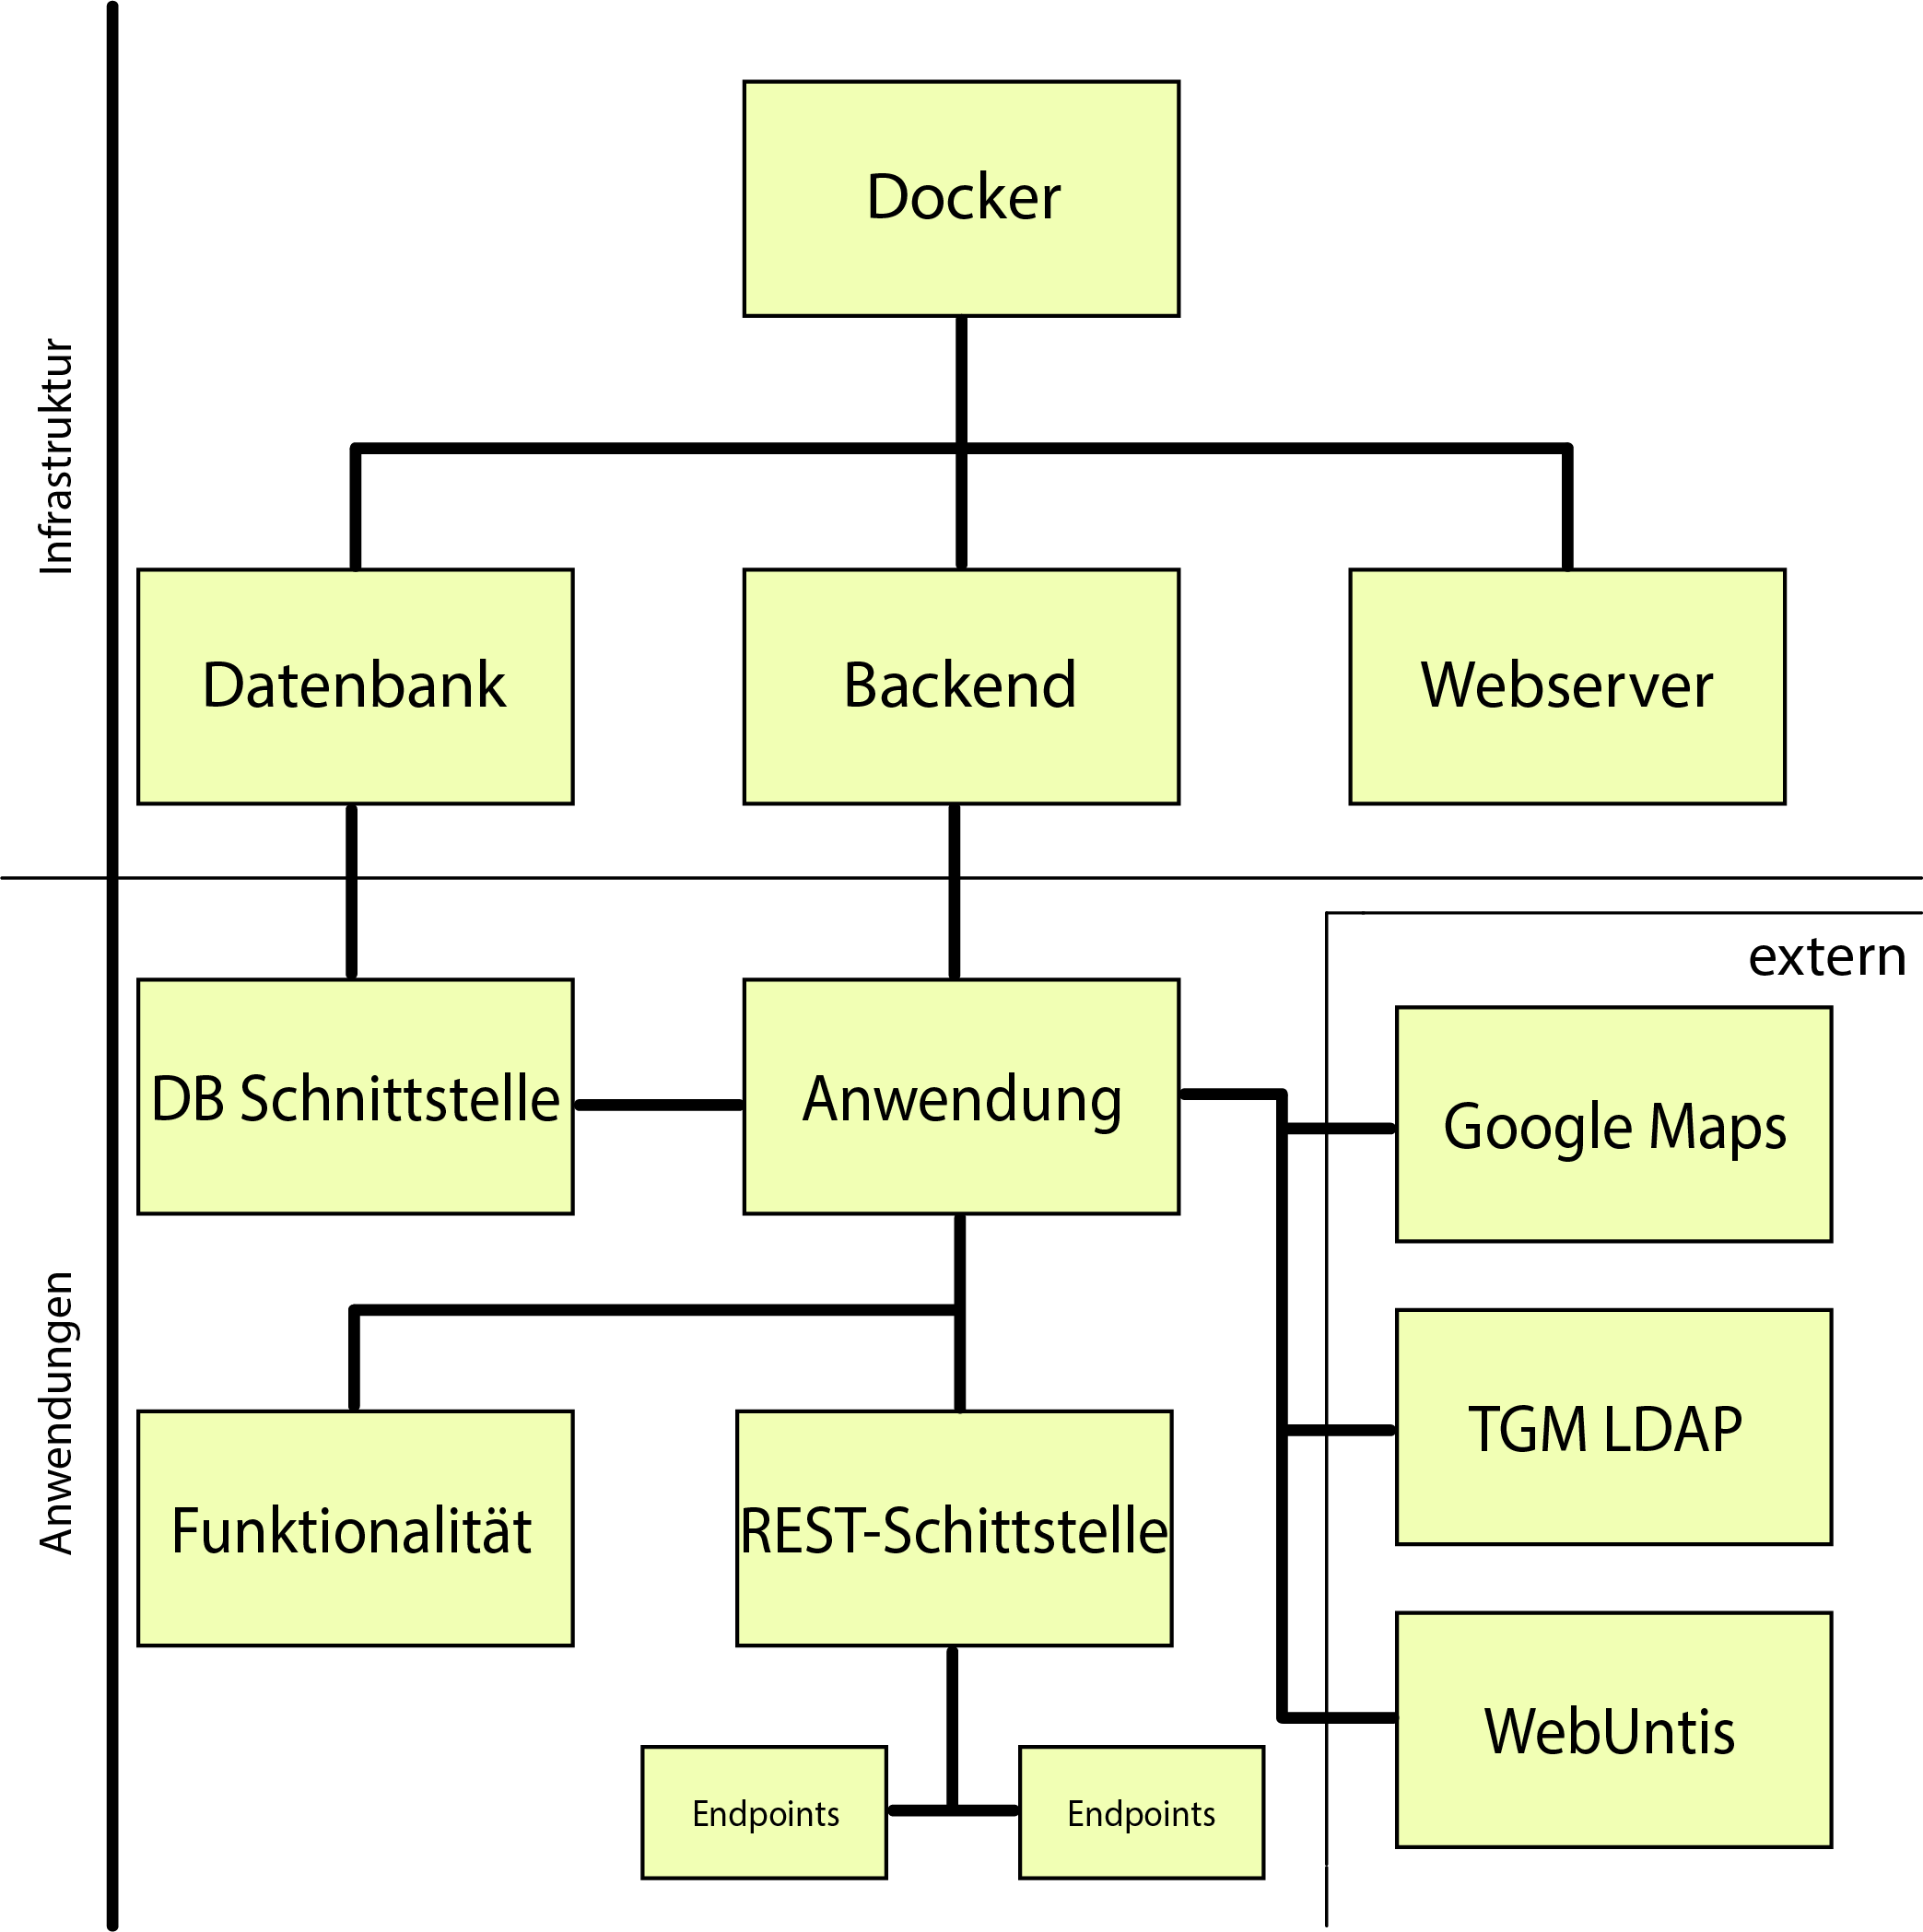
\includegraphics[width=0.8\linewidth]{images/uebersicht}
		\caption[Übersicht über die Komponenten]{Übersicht über die verschiedenen Komponenten der Infrastruktur und der Anwendung}
		\label{fig:uebersicht}
	\end{figure}
	
	\newpage
	In den folgenden Kapiteln werden die aktuell verfügbaren Technologien, welche für die Umsetzung im Backendbereich in Frage kommen, beschrieben und gegebenenfalls - sofern mehrere sinnvolle Kandidaten vorhanden sind - auch verglichen. Auf einen detaillierten Vergleich jeglicher verwendbaren Third Party Packages, welche dazu genutzt werden könnten, um die Funktionalität im Backend zu implementieren, wird auf Grund der extrem hohen Anzahl im Sinne der Übersichtlichkeit verzichtet. Unter die benutzten Packages, fallen jedenfalls Module wie maroto (zum Erstellen von PDF-Dateien \cite{maroto}), excelize (zum Erstellen von Excel-Dateien \cite{excelize}) und jwt-go (zum Erstellen von \Gls{jwt} \cite{jwt-go}) 
	\subsection{Docker}
	Um die Infrastruktur des Projektes einfach aufbauen zu können, wird \Gls{docker} genutzt. Da es sich hier um eine komplex strukturierte Infrastruktur handelt, wird zusätzlich das Werkzeug \Gls{dcompose} genutzt. Mit Docker Compose kann eine Infrastruktur aufgebaut werden, die der \hyperref[fig:uebersicht]{Abbildung 5.2} entspricht. Für diese sind folgende Container vorgesehen, die in den nächsten Kapiteln noch im Detail beschrieben werden.
		\subsubsection{Datenbank}
		\label{sec:db}
		Um die Daten, die durch Refundable erhoben und generiert werden, zu speichern, wird eine \gls{db} benötigt. Auf Grund der Daten, welche sich durch unterschiedliche Datenstrukturen auszeichnen, ist der Einsatz einer \gls{relDb} nicht sinnvoll. Stattdessen empfiehlt sich die Verwendung einer \gls{nosqlDb}.
		Standardmäßig wird zwischen 4 verschiedenen Typen von NoSQL Datenbanken unterschieden, welche jeweils nur in ihrem eigenen Use Cases sinnvoll anwendbar sind \cite{nosqltypes}:
		\begin{itemize}
			\item Key-Value Datenbank
			\item spaltenorientierte Datenbank
			\item graphenorientierte Datenbank
			\item dokumentenorientierte Datenbank
		\end{itemize}
		\captionof{listing}{NoSQL Datenbank-Typen}
		\label{code:nosqltypes}~\\	
		Bei Key-Value Datenbanken wird einem Schlüssel ein Wert hinterlegt. Dieser Wert ist dann jederzeit über den Schlüssel in der Datenbank abrufbar. Für unseren Use Case ist dieses System nicht sinnvoll anzuwenden, da die von uns benutzten Daten hierfür zu komplex im Aufbau sind.~\\
		Bei spaltenorientierten Datenbanken werden Daten vorrangig über ihre Spalten (statt wie bei relationalen \gls{db}s in Zeilen) analysiert. Dies ermöglicht die einfache Umsetzung statistischer Methoden auf Basis der Spalten. Da jedoch wieder eine Tabelle als Grundstruktur vorliegt, ist dieser Typ von Datenbank nicht sinnvoll anwendbar für Refundable.~\\
		Bei graphenorientierten Daten wird die Beziehung zwischen einzelnen Elementen hervorgehoben. Daten werden hier in Knoten gespeichert, welche zu anderen verbunden werden können. Die primären Elemente sind hierbei die Beziehungen, anstatt der Daten selbst. Da die Daten von Refundable nicht über starke Beziehungen charakterisiert sind, ist auch dieser Datenbank-Typ nicht sinnvoll zu benutzen.~\\		
		Zuletzt bei dokumentenorientierten Datenbanken unterliegt jeder Datensatz in einem eigenen Dokument, welches in \Gls{json}, \Gls{yaml}, \Gls{xml} oder ähnlichen Datenformaten gespeichert wird. Dadurch ist auch eine jeweils von einander unabhängige Datenstruktur möglich. Auf Grund der Flexibilität bei Datenstrukturen ist eine dokumentenorientierte Datenbank eindeutig sinnvoll zu verwenden.~\\
		Als \gls{dbms} kommt bei dieser Auswahl einige Software in Frage. Die am meisten verbreitete Software hier ist MongoDB und CouchDB \cite{mongo}. Wo MongoDB auf strenge \gls{konsistenz} setzt, setzt CouchDB auf hohe \gls{verfugbarkeit}. Da in unserem Projekt Konsistenz wichtiger ist als Verfügbarkeit wird MongoDB in einem Container als Datenbankmanagementsystem verwendet.
		
		\subsubsection{Backend-Container}
		
		Ebenfalls wird ein Container, also eine Umgebung, in dem das Backend laufen kann, erstellt. Dieser wird direkt zu den anderen Containern hinzugefügt, damit dieser über ein Docker-Netzwerk mit den anderen Containern kommunizieren kann.~\\
		Um diesen Container zu realisieren wird als Basis ein golang-Image genutzt \cite{golang}. Dieses stellt eine sehr sparsame Linux-Instanz dar, welche mit einer golang-Umgebung ausgestattet ist. Um diesen Container noch entsprechend anzupassen, wird ein entsprechendes Docker-Image über ein Dockerfile gebaut.
		
		\subsubsection{Webserver}
		
		Als Webserver wird ein Apache2 Server genutzt \cite{apache}. Der Service stellt hierbei das Webinterface (Frontend) im Internet zur Verfügung. Dieser Container ruft automatisch das Frontend auf und kopiert es in seine Umgebung. Ebenfalls muss der Container Zugriff auf Zertifikaten bekommen, um einen sicheren Zugriff über \gls{https} gewährleisten zu können.
				
	\subsection{Deployment}
	
	Das Deployment soll automatisch geschehen. Um dies einfach zu ermöglichen, werden die oben zuvor beschriebenen Docker-Container, GitHub und ein Skript, welches die Schritte ausführt, genutzt. Das Skript ist hier der Hauptbaustein, welcher den Vorgang startet und steuert. Zusätzlich zum Installationsvorgang, soll das Skript auch die weitere Steuerung der Software, also starten, stoppen, updaten, cleanen und deinstallieren, beinhalten.~\\
	Das Skript liegt in einem eigenem Install-\Gls{repo}, in welchem sonst keine weiteren Dateien liegen. Dadurch kann es einfach geklont und direkt installiert werden; die restlichen Installations-Schritte werden automatisch erledigt.~\\
	Da das Deployment auf einer Linux-Maschine ermöglicht werden soll, wird \Gls{bash} als Standard-Skriptsprache benutzt. Zur Verteilung des Scripts wird, wie erwähnt, \Gls{git} mit dem Online Repository-Hosting Service \Gls{github} verwendet.
	\subsection{REST-Schnittstelle}
	Bei einer REST-Schnittstelle handelt es sich um einen bestimmten Aufbau einer Softwareschnittstelle bei verteilten Systemen \cite{Patni2017}. Das hierbei angewendete Prinzip nennt sich \enquote{Representational State Transfer} (kurz REST). Es zeichnet sich durch folgende Eigenschaften aus:
	\begin{itemize}
		\item \textbf{Client-Server}, wobei es um eine strikte Trennung zwischen dem Client (dem REST-Client) und dem Server (der REST-Schnittstelle, als Webservice) geht
		\item \textbf{Stateless}, wobei es um die Zustandslosigkeit des Servers geht. Das heißt, dass der Server sich keinerlei Zustände der Clients merkt.
		\item \textbf{Caching}: Der Server speichert die Responses zwischen. Dadurch kann die Latenzzeit minimiert werden, da Daten öfters zurückgegeben werden, anstatt sie jedes Mal erneut berechnen zu müssen.
		\item \textbf{Einheitliche Schnittstelle} bedeutet, dass die Schnittstelle ein einheitliches Datenformat verwendet, um via HTTP über CRUD-Methoden (Create, Read, Update, Delete) zu kommunizieren.
		\item \textbf{Layer-System} bedeutet, dass die Schnittstelle, als Webservice so designed wird, dass auch weitere Schichten, wie Gateways und Proxies, transparent dazwischen aufgebaut werden können.
		\item \textbf{Code-on-demand} (optional): Hierbei besteht die Möglichkeit ausführbaren Code an die Clients zu schicken, sodass diese den dann ausführen können.
	\end{itemize}
	\captionof{listing}{Prinzipien des Representation State Transfer}
	\label{code:rest}
		\subsubsection{Java und Spring}
		Java ist eine der bekanntesten Programmiersprachen. Sie zeichnet sich durch Plattform-Unabhängigkeit aus \cite{jdkDocs}. Um dies zu erreichen, wird Bytecode von einem eigenem Programm, der Java Virtual Machine, interpretiert. Java arbeitet objektorientiert und ist statisch typisiert. Dies bedeutet, dass bereits vor dem Ausführen die Datentypen definiert sind. Java unterstützt auch Multithreading. Um einfach eine REST-Schnittstelle in Java bauen zu können, wird Spring Boot genutzt \cite{springDocs}. Die Verwendung von Spring ermöglicht Webapps, Tasks oder Microservices einfacher umzusetzen. Prinzipiell arbeitet Spring asynchron und flexibel, sodass es einfach zu skalieren ist. 
		
		\subsubsection{Python und Flask}
		Um mit Python eine REST-Schnittstelle zu realisieren muss auf das Package (Framework) Python Flask zurückgegriffen werden \cite{flaskDocs}. Flask wird hierbei dazu genutzt, um den Webservice zu bauen. Python und Java unterscheiden sich prinzipiell sehr. Python ist im Gegensatz zu Java dynamisch typisiert, dies bedeutet, dass eine Variablendeklaration nicht notwendig ist und der Datentyp einer Variable erst zur Laufzeit klar ist \cite{pythonDocs}. Anders als Java setzt Python auf Third-Party Packages, welche sehr einfach importiert werden können. Durch die große Community Pythons ist ein Großteil der Tools, die man benötigt, meist schon vorprogrammiert und kann einfach importiert werden. Zusätzlich ist der Syntax (speziell was Zeichensetzung anbelangt) einfacher zu verstehen, als jener von Java.
		
		\subsubsection{Golang}
		\label{chapter:golanganalyse}
		Golang (kurz Go) ist eine von Google entwickelte und publizierte Programmiersprache \cite{goDocs}. Sie wurde aus der Unzufriedenheit über Java, C++ und Python heraus entwickelt, welche am häufigsten bei Google eingesetzt wurden. All diese Programmiersprachen haben Nachteile in Googles Business Case, deswegen wurde Go speziell für skalierbare Netzwerkdienste und Cloud Computing entwickelt. Aus diesem Grund besitzt Go auch eine native Möglichkeit für den einfachen Aufbau von REST-Schnittstellen. Da bei der Entwicklung von Go speziell aus den Fehlern in Performance und Sprachdesign aus anderen Sprachen gelernt wurde, verbindet Go die Vorteile der anderen Sprachen. Darunter fallen die starke und statische Typisierung, Objektorientierung, Pointer und eine verbesserte Compiler-Effizienz.
		\newpage
		\subsubsection{Vergleich}
		Diese drei Sprachen werden nun in den Aspekten der Performance, dem Sprachdesign, der Komplexität des Aufbaus einer REST-Schnittstelle, das Vorhandensein von Frameworks, die Erfahrung des Teams und eine vorhandene ausführliche Dokumentation analysiert und verglichen. Hierbei wird auf einer Punkteskala von 0 - 9 bewertet.
		\captionof{table}{Vergleich zwischen Java, Python und Golang}\label{tbl:comparisonlang}
		\begin{table}
			\begin{tabular}{|l|r|r|r|r|r|r|r|}
				\hline
				\multicolumn{1}{|c|}{\textbf{Kriterien}} & \multicolumn{1}{c|}{\textbf{Gewichtung}} & \multicolumn{2}{c|}{\textbf{Java und Spring}} & \multicolumn{2}{c|}{\textbf{Python und Flask}} & \multicolumn{2}{c|}{\textbf{Golang}} \\ \cline{3-8} 
				& \multicolumn{1}{l|}{} & \multicolumn{1}{c|}{Punkte} & \multicolumn{1}{c|}{Wertung} & \multicolumn{1}{c|}{Punkte} & \multicolumn{1}{c|}{Wertung} & \multicolumn{1}{c|}{Punkte} & \multicolumn{1}{c|}{Wertung} \\ \hline
				Performance & 15\% & 6 & 0,9 & 3 & 0,45 & 9 & 1,35 \\ \hline
				Sprachdesign & 25\% & 6 & 1,5 & 4 & 1 & 8 & 2 \\ \hline
				\begin{tabular}[c]{@{}l@{}}Aufbau einer \\ REST-Schnittstelle\end{tabular} & 5\% & 7 & 0,35 & 8 & 0,40 & 9 & 0,45 \\ \hline
				\begin{tabular}[c]{@{}l@{}}Vorhandensein von\\ Frameworks\end{tabular} & 15\% & 7 & 1,05 & 9 & 1,35 & 9 & 1,35 \\ \hline
				\begin{tabular}[c]{@{}l@{}}Erfahrung des \\ Teams\end{tabular} & 20\% & 4 & 0,8 & 3 & 0,6 & 6 & 1,2 \\ \hline
				Dokumentation & 20\% & 8 & 1,6 & 7 & 1,4 & 9 & 1,8 \\ \hline
				\textbf{Summe} & 100\% & \multicolumn{1}{l|}{} & \multicolumn{1}{c|}{\textbf{6,2}} & \multicolumn{1}{c|}{\textbf{}} & \multicolumn{1}{c|}{\textbf{5,2}} & \multicolumn{1}{c|}{\textbf{}} & \multicolumn{1}{c|}{\textbf{8,15}} \\ \hline
			\end{tabular}
		\end{table}
		~\\
		Daraus und aus der durchgeführten Recherche, lässt sich schließen, dass Golang sich speziell bei den Punkten Performance und Sprachdesign durchsetzen kann. Ansonsten schneiden die verschiedenen Sprachen inklusive der teilweise benötigten Frameworks großteils ähnlich hoch ab. Zusammenfassend eignet sich die Verwendung von Golang am Besten als Programmiersprache für unser Projekt, da sie im numerischen Vergleich mit der höchsten Punktezahl abschnitt, aber auch durch die speziellen Hintergründe ihrer Entwicklung genau zu den Voraussetzungen passt.
	\subsection{Kommunikation und Datenformate}
	Wie bereits erwähnt, zeichnen sich REST-Schnittstellen unter anderem dadurch aus, dass sie ein einheitliches Datenformat voraussetzen. Aus diesem Grund stellen sich die Fragen: \\~\\
	Welche Datenformate eignen sich für einen konsistenten und performanten Datenaustausch zwischen Datenbank, REST-Schnittstelle und Client? \\~\\
	Welche Vor- und Nachteile bringen diese im Hinblick auf Performance, Softwarewartung und -evolution?\\~\\
	Um diese Fragen zu beantworten werden in den nächsten Kapiteln entsprechende Datenformate vorgestellt, beschrieben und analysiert.
	
	\newpage
		\label{sec:json}
		\subsubsection{JSON}
		\Gls{json} (JavaScript Object Notation) ist ein Textformat, welches für die Serialisierung von Daten genutzt werden kann \cite{rfc4627}. 
		Es umfasst 6 Datentypen, davon 4 Primitive und 2 Strukturen:
		\begin{itemize}
			\item \Gls{string}s
			\item Zahlen
			\item \Gls{bool}s
			\item \Gls{null}
			\item \Gls{array}s
			\item \Gls{object}e
		\end{itemize}
		\captionof{listing}{JSON - Datentypen}
		\label{code:jsontypes}~\\	
		Wie so eine Serialisierung aussieht, wird in folgendem Beispiel ersichtlich: 
		
		\begin{code}{json}
		{
			"classes": [
				{
					"name": "1AHIT",
					"lastYear": false,
					"students": 35,
					"class-rep": "Michaela Musterfrau"
				},
				{
					"name": "5BHIT",
					"lastYear": true,
					"students": 25,
					"class-rep": "Maximilian Frühmann"
				}
			],
			"date": "2021-09-01"
		}
		\end{code}
		\captionof{listing}{JSON Beispiel}
		\label{code:json}~\\
		Das in \hyperref[code:json]{Auflistung 5.8} stehende Beispiel stellt ein Objekt mit zwei Feldern dar. Das erste Feld ist ein \enquote{classes}-Array, welches verschiedene Schulklassen beinhaltet. Diese Schulklassen haben jeweils einen String als Namen, einen Boolean als Feld, das angibt, ob es sich um eine Abschlussklasse handelt, die Anzahl der Schüler als Zahl und den Namen des Klassensprechers. Nachdem die Definition des Arrays abgeschlossen ist, wird noch ein weiteres Feld im obersten Objekt angegeben, welches das aktuelle Datum als String beinhaltet.
		\\~\\
		Der JSON-Standard umfasst genaue Regeln, wie mit den Datentypen, speziell mit Strings und Zahlen, umzugehen ist \cite{rfc4627}.
		Über einen JSON-Generator kann ein JSON-Text auf Basis eines Dateninputs generiert werden. Wenn die Daten aus dem JSON-Textformat wieder extrahiert werden sollen, spricht man vom \enquote{parsen} von Daten.\\
		Jede moderne Programmiersprache hat einen eigenen JSON-Parser implementiert oder es ist möglich einen über ein \Gls{tpp} zu laden.
		\subsubsection{XML}
		\Gls{xml} (Extensible Markup Language) ist ein strukturiertes textbasiertes Datenformat \cite{xmlStandard}. Es handelt sich hierbei um eine Markup-Language. Als Syntax von XML werden Tags verwendet. Ein <Tag> ist ein Anfangs-Tag und ein </Tag> ein End-Tag. Ebenfalls können Attribute in einem Anfangs-Tag definiert werden (<Tag attribut=\dq wert\dq ). XML-Dateien brauchen im Gegensatz zu JSON-Texten ein Wurzelelement.
		\begin{code}{xml}
		<school>
			<classes>
				<class lastYear="false" students="35" class-rep="null">1AHIT</class>
				<class lastYear="true" students="25" class-rep="null">5BHIT</class>
			</classes>
			<date>2021-09-01</date>
		</school>
		\end{code}
		\captionof{listing}{XML Beispiel}
		\label{code:xml}~\\
		Das Beispiel definiert ein Wurzelelement für die Datenstruktur namens \enquote{school}. Dieses hat ein Kindelement \enquote{classes}. In diesem sind einzelne \enquote{class}-Tags mit den nötigen Attributen und dem Namen der Klasse innerhalb der Tags. Dies wird als Alternative für die in XML nicht vorhandenen Arrays genutzt. Zuletzt wird wieder ein untergeordnetes \enquote{date}-Element mit dem aktuellem Datum als Inhalt hinzugefügt.\\~\\
		Das XML-Dateiformat kann entweder gültig oder wohlgeformt sein \cite{xmlStandard}. Dies beschreibt die Einhaltung des Syntax und der Regeln des XML Standards.\\
		Des Weiteren besteht die Möglichkeit die Struktur von XML-Dateien anhand der XML-Schema-Sprache oder durch die Document Type Definition zu beschreiben. XML Dateien brauchen aus diesen Gründen unbedingt einen Parser für die Umwandlung.
		
		\newpage
		
		\subsubsection{CSV}
		CSV (Comma-Separated Values) ist ein Textformat, mit welchem man Tabellen textbasiert darstellen kann \cite{rfc4180}. Hierbei werden Spalten durch \dq , \dq  ~(Beistriche) getrennt und Zeilen durch einen Zeilenumbruch (CRLF; LF). Die erste Zeile repräsentiert die Namen der Spalten. Eine Beschreibung einer Tabelle mit CSV sieht wie folgt aus:
		\begin{code}{python}
			Class,lastYear,students,class-rep
			1AHIT,false,35,null
			5BHIT,true,25,null
		\end{code}
		\captionof{listing}{CSV Beispiel}
		\label{code:csv}~\\
		Im Beispiel werden die beiden Klassen als zwei Datensätze in einer Tabelle aufgelistet. Auf Grund der Struktur von CSV ist es nur möglich den Array-Teil des Objektes darzustellen. Ansonsten ist der CSV-Standard recht simpel gehalten. Der letzte Punkt auf den der Standard hierbei eingeht ist, dass "-Zeichen um die Daten gesetzt werden können \cite{rfc4180}. Sollten, diese nicht geschlossen werden kann es jedoch zu unvorhersehbaren Verhalten kommen.
		\subsubsection{Vergleich}
		Ein Vergleich zwischen den Datenformaten JSON, XML und CSV ist auf dem ersten Blick nicht zielführend. Wie aus den einzelnen Beschreibungen der Technologien oben entnommen werden kann, handelt es sich beim CSV-Format um Tabellen. Bereits bei der \hyperref[sec:db]{Wahl der dokumentenorientierten Datenbank MongoDB} war der Hintergedanke relationale Datenbanken und ihrer Speicherstruktur, Tabellen, weitestmöglich zu vermeiden. 
		
		Wenn man sich nun auch das CSV Format und speziell das \hyperref[code:csv]{Beispiel} anschaut, merkt man, dass die Umwandlung des ursprünglichen Objektes nur indirekt möglich war und als Auflistung der Klassen endete. Das Resultat ist, dass Objekte zu CSV-Tabellen mit vielen Spalten und einer Zeile werden und Arrays zu Tabellen mit wenigen Spalten und vielen Zeilen. Eine Darstellung beider Datentypen in einer Tabelle ist nicht möglich. Dies disqualifiziert CSV für den Einsatz als Datenformat im Projekt.
		
		Vergleicht man nun JSON und XML so scheinen diese erst ähnlich. Jedoch besteht bei XML keine Möglichkeit Arrays zu definieren. Des Weiteren wird XML nicht nur als Datenformat zur Kommunikation genutzt, sondern hat noch weitere Nutzen als Markup Language. Demnach ist XML sehr überladen, speziell deswegen weil es einen eigenen speziellen XML-Parser braucht.
		
		Auch JSON braucht einen sogenannten Parser, jedoch handelt es sich hierbei nur um das Einlesen des JSON-Textes und dem Generieren des Objekts. Eine Validierung wie in XML bleibt aus. Zuletzt ist JSON nicht nur schneller, sondern auch effizienter was den Verbrauch an CPU-Leistung und an Arbeitsspeicher angeht \cite{Nurseitov}.
		
		Aus diesen Gründen wird JSON als Datenformat zur Kommunikation zwischen den einzelnen Komponenten Refundables genutzt werden.